\documentclass[12pt]{article}
\usepackage[margin=1in]{geometry}
\usepackage{datetime}
\usepackage[T1]{fontenc}
\usepackage{titling}
\usepackage{titlesec}
\usepackage{hyperref}
%\usepackage{natbib}
\usepackage{graphicx}
\usepackage{tikz}
\usepackage{caption}
\usepackage{subcaption}
\usepackage{float}
\usepackage[parfill]{parskip}

\titleformat{\section}[runin]
  {\normalfont\Large\bfseries}{\thesection}{1em}{}
\titleformat{\subsection}[runin]
  {\normalfont\large\bfseries}{\thesubsection}{1em}{}
  
\renewcommand{\thesection}{\Roman{section}} 
\renewcommand{\thesubsection}{\thesection.\Roman{subsection}}

\makeatletter

\renewcommand{\maketitle}{\bgroup\setlength{\parindent}{0pt}
\begin{flushleft}
  \textbf{\Large \@title}\newline
  
  \@author\\
  Date: \@date
\end{flushleft}\egroup
}
\makeatother

\author{Author: Tingfeng Xia, University of Toronto, \url{mailto:tingfeng.xia@mail.utoronto.ca}}
\title{\textbf{Bufferbloat Problem} \\ {\small CSC458 Computer Networks Programming Assignment 2}}

\date{\today}

\begin{document}
\maketitle
\section*{Abstract} 
Bufferbloat refers to the existence of excessively large and frequently full buffers inside a network. \cite{sivov12} 

Most TCP congestion control algorithms rely on packet drops to determine the available bandwidth between two ends of a connection.\cite{allman09, sayad11} In general, TCP congestion control algorithms speed up the data transfer until packets start to drop, then slow down the transmission rate. Under ideal conditions, we expect an equilibrium speed to be reached after a period of time of adjustments.

To illustrate the problem of Bufferbloat, let's consider an internet topology illustrated in Figure \ref{fig;topology}. From our perspective, $h_1$ to $s_0$ via $\ell_1$ should be sending at maximum 10Mbps to avoid congestion, since $\ell_2$ is the bottleneck in our network with a link speed of 10Mbps. However, from $h_1$'s perspective, it only knows to decrease data transfer speed when it  receives signal of packet drop, which will happen after the buffer of $s_0$ is full. Importantly, $h_1$ will not slow down its data transfer speed until $s_0$  buffer is saturated and $s_0$ begins to drop packets from $h_1$. In other words, the buffer within $s_0$ caused packet drop signals cease to be a timely indication of congestion, which TCP congestion avoidance algorithms rely heavily on. 

Bufferbloat causes increase in queueing delay, and thus causes end users to experience increase in latency, which is the sum of transmission delay, processing delay, and queueing delay. \cite{sivov12} Bufferbloat also causes jitters and decreases the overall throughput of the network. 

\begin{figure}[h]
	\begin{center}
	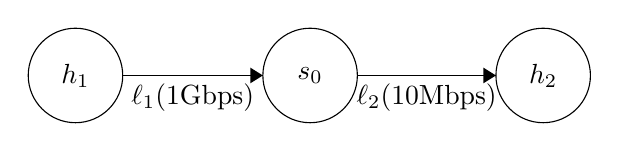
\begin{tikzpicture}[scale=0.2]
	\tikzstyle{every node}+=[inner sep=0pt]
	\draw [black] (3.2,-3.2) circle (3);
	\draw (3.2,-3.2) node {$h_1$};
	\draw [black] (18.1,-3.2) circle (3);
	\draw (18.1,-3.2) node {$s_0$};
	\draw [black] (32.9,-3.2) circle (3);
	\draw (32.9,-3.2) node {$h_2$};
	\draw [black] (6.2,-3.2) -- (15.1,-3.2);
	\fill [black] (15.1,-3.2) -- (14.3,-2.7) -- (14.3,-3.7);
	\draw (10.65,-3.7) node [below] {$\ell_1$(1Gbps)};
	\draw [black] (21.1,-3.2) -- (29.9,-3.2);
	\fill [black] (29.9,-3.2) -- (29.1,-2.7) -- (29.1,-3.7);
	\draw (25.5,-3.7) node [below] {$\ell_2$(10Mbps)};
	\end{tikzpicture}
	\end{center}
	\captionsetup{format=hang}
	\caption{\label{fig;topology}Assignment Topology. Link $\ell_1$ and $\ell_2$ has bandwidths 1Gbps and 10Mbps respectively; Router $s_0$ has buffer size 150kB, and assuming MTU of 1500 bytes it can buffer approximately 100 packets. }
\end{figure}
\section*{Methods} 
We emulate our Assignment topology, as illustrated in Figure \ref{fig;topology}, internet topology using mininet. Then, we simultaneously perform the following three tasks
\begin{itemize}
	\setlength\itemsep{-0.5em}
	\item start a long lived TCP flow sending data from $h_1$ to $h_2$, and
	\item send 1 ping per 0.1 second from $h_1$ to $h_2$, and 
	\item spawn an web server on $h_1$, and download the webpage from $h_1$ once every two seconds. 
\end{itemize}
This simulation is repeated for three different queue sizes, $Q = 5 / 20 / 100 $ pkts. Then, for each max queue size, we plot the time-series of the long-lived TCP flow's cwrd, the RTT reported by ping, the webpage download time, and the queue size at the router $s_0$. 

\section*{Results}
\begin{figure}[H]
	\center\begin{subfigure}[b]{0.5\textwidth}
		\includegraphics[width=\textwidth]{../bb-q5/cwnd-iperf}
		\caption{\label{fig:buffer5cwrd}Long-lived TCP flow's cwrd}
	\end{subfigure}
	\begin{subfigure}[b]{0.49\textwidth}
		\includegraphics[width=\textwidth]{../bb-q5/rtt}
		\caption{\label{fig:buffer5rtt}RTT repoted by ping}
	\end{subfigure}
	\begin{subfigure}[b]{0.5\textwidth}
		\includegraphics[width=\textwidth]{../bb-q5/download}
		\caption{\label{fig:buffer5download}Webpage download time}
	\end{subfigure}
	\begin{subfigure}[b]{0.49\textwidth}
		\includegraphics[width=\textwidth]{../bb-q5/q}
		\caption{\label{fig:buffer5q}Queue size at the router}
	\end{subfigure}
	\captionsetup{format=hang}
	\caption{\label{fig:buffer5}Long-lived TCP flow's cwrd, RTT reported by ping, webpage download time, and queue size at the router with max buffer size of 5. }
\end{figure}
\begin{figure}[H]
	\center\begin{subfigure}[b]{0.5\textwidth}
		\includegraphics[width=\textwidth]{../bb-q20/cwnd-iperf}
		\caption{\label{fig:buffer20cwrd}Long-lived TCP flow's cwrd}
	\end{subfigure}
	\begin{subfigure}[b]{0.49\textwidth}
		\includegraphics[width=\textwidth]{../bb-q20/rtt}
		\caption{\label{fig:buffer20rtt}RTT repoted by ping}
	\end{subfigure}
	\begin{subfigure}[b]{0.5\textwidth}
		\includegraphics[width=\textwidth]{../bb-q20/download}
		\caption{\label{fig:buffer20download}Webpage download time}
	\end{subfigure}
	\begin{subfigure}[b]{0.49\textwidth}
		\includegraphics[width=\textwidth]{../bb-q20/q}
		\caption{\label{fig:buffer20q}Queue size at the router}
	\end{subfigure}
	\captionsetup{format=hang}
	\caption{\label{fig:buffer20}Long-lived TCP flow's cwrd, RTT reported by ping, webpage download time, and queue size at the router with max buffer size of 20. }
\end{figure}
\begin{figure}[H]
	\center\begin{subfigure}[b]{0.5\textwidth}
		\includegraphics[width=\textwidth]{../bb-q100/cwnd-iperf}
		\caption{\label{fig:buffer100cwrd}Long-lived TCP flow's cwrd}
	\end{subfigure}
	\begin{subfigure}[b]{0.49\textwidth}
		\includegraphics[width=\textwidth]{../bb-q100/rtt}
		\caption{\label{fig:buffer100rtt}RTT repoted by ping}
	\end{subfigure}
	\begin{subfigure}[b]{0.5\textwidth}
		\includegraphics[width=\textwidth]{../bb-q100/download}
		\caption{\label{fig:buffer100download}Webpage download time}
	\end{subfigure}
	\begin{subfigure}[b]{0.49\textwidth}
		\includegraphics[width=\textwidth]{../bb-q100/q}
		\caption{\label{fig:buffer100q}Queue size at the router}
	\end{subfigure}
	\captionsetup{format=hang}
	\caption{\label{fig:buffer100}Long-lived TCP flow's cwrd, RTT reported by ping, webpage download time, and queue size at the router with max buffer size of 100. }
\end{figure}


\section*{Discussion}












\bibliographystyle{apalike}
\bibliography{bib.bib}

\end{document}
